\chapter{Projekt}
Jednotlivé sekce přílohy byly vytvořeny za účelem doplnění zbývajících bodů požadavků předmětu Elektronické publikace. Ostatní požadavky již byly splněny v rámci samotného textu práce.

% Doplnění - zvýrazňování textu
\section{Zvýrazňování textu}
\textsc{Text psaný kapitálkami}



% Doplnění - výčtová prostředí
\section{Výčtová prostředí}
\begin{enumerate}
    \item První
    \item Druhý
    \item Třetí
\end{enumerate}

\newcounter{ListCounter}
\begin{list}{Část \Roman{ListCounter}:}{\usecounter{ListCounter}}
    \item Úvod
    \item Vypracování
    \item Závěr
\end{list}



% Doplnění - komentáře
\section{Komentáře}
\begin{comment}
    {\LARGE Obrovský text, který ale není vidět}
    \textit{Stejně tento vložený soubor!}
    \chapter{Úvod}
\label{chap:1}
Motivací práce bylo vytvořit moderní responzivní webovou aplikaci pro sdílení virtuální tabule, která bude umožňovat spolupráci více uživatelů na různých typech zařízení.
Virtuální tabule slouží k zaznamenávání a sdílení návrhů a ilustrací pomocí jednoduchých nástrojů, díky kterým je možné ji využít v práci, škole či v osobním životě.
%je oblast využití tohoto řešení skutečně široká.
Samotný obsah tabule je průběžně synchronizován, takže jsou změny jednotlivých uživatelů vidět přímo bez nutnosti stránku aktualizovat.
Zároveň jsou také veškeré úpravy ukládány do databáze, která slouží jako trvalé uložiště dat a také záloha při případném výpadku serveru či spojení.
%Databáze je poté využita pro načítání obsahu při připojení uživatele a také jako záloha při případném výpadku serveru či spojení.

%Myšleno je také na případné problémy, které se mohou vyskytnout nejen na straně uživatele, ale také na straně serveru.
%Samotný obsah tabule je průběžně synchronizován a ukládán, takže při výpadku sítě či serveru je po obnovení spojení vždy načten poslední uložený stav.
%, tak aby při , každopádně toto řešení nabízí také export pomocí obrázku či zdrojového souboru, kdykoli možné 
První kapitola se věnuje výběru jednotlivých stávajících řešení nástrojů pro sdílení virtuální tabule.
Kapitola uvádí nástroje a technologie vybraných webů a porovnává je s vypracovaným řešením.

Druhá kapitola se zaměřuje na rozbor požadavků, analýzu problémů a možných řešení a také na architekturu systému.
Kapitola přibližuje vnitřní strukturu systému na kterém je celé řešení postaveno.

Třetí kapitola pak pojednává o implementaci samotného řešení a jeho jednotlivých součástí.
Nejprve je zmíněno vykreslování, jeho optimalizace pomocí vláken a také zpracování barev v rámci barevných motivů.
Dále se kapitola věnuje výměně dat mezi klientských zařízením a serverem pomocí WebSockets.
Následně je popsána správa dat, která na lokální či serverové úrovni zajišťuje využití dat pro konkrétní potřeby uživatele.
Zmíněno je mimo jiné využití MySQL databáze, LocalStorage a Fetch API a také jednotlivé možnosti exportování tabule do rastrové či nativní podoby.
V poslední řadě se kapitola věnuje uživatelskému rozhraní z pohledu responzivity, podpory více jazyků včetně jejich zakomponování do sdílení tabule a také jednotlivým stránkám a jejich podobě ve finálním řešení.
%, ať už lokální či serverová zahrnuje využití MySQL databáze, LocalStorage či Fetch API a je pak dále včetně exportu tabule detailně popsána.
%S daty se lokálně i na serveru dále pracuje a tento proces je pak dále popsán včetně využití MySQL databáze, LocalStorage či Fetch API.  jsou následně ukládána do MySQL databáze či LocalStorage, což je také podrobně popsáno.
%Serverová i lokální správa dat je pak dále popsána včetně využití MySQL databáze a LocalStorage.
%začátek vývoje řešení, kdy 
%pojednává o využití Canvas API, coby plnohodnotné technologie pro vykreslování grafického výstupu na webu.
%Kapitola obsahuje popis této technologie včetně ukázky několika příkladů základních funkcí.

%Třetí kapitola se zaměřuje na výměnu dat mezi klientským zařízením a serverem pomocí protokolu WebSocket.
%Tento protokol poskytuje snadný a spolehlivý přenos dat, což umožňuje interaktivní spolupráci více uživatelů.

%Čtvrtá kapitola se věnuje správě dat a popisuje dva základní způsoby jak lze data ukládat či načítat pro další využití.
%Popsáno je využití MySQL databáze, kde data zůstávají uloženy dlouhodobě mezi jednotlivými návštěvami webu a dále pak exportování a nahrání dat v nativní podobě ve formátu JSON.

%Pátá kapitola rozšiřuje předchozí kapitoly o pohled na optimalizaci jednotlivých příkazů a dat, což umožňuje plynulejší chod webové aplikace.
%Zmiňuje se mimo jiné o Web workers použitých k rozdělení instrukcí do více vláken či o různých změnách v datech pro konkrétní místa použití.

%Poslední kapitola se zaměřuje na nedokončené části bakalářské práce a jejich možné rozšíření či vylepšení.
\endinput
\end{comment}



% Doplnění - vkládání vzorců
\section{Vkládání vzorců}
\begin{equation}
    E = mc^2
\end{equation}



% Doplnění - sazba indexu
\section{Sazba indexu}
Tento text je napsán v jazyce \LaTeX\index{\LaTeX}, který slouží k sazbě\index{sazba} dokumentu formy bakalářské práce\index{bakalářská práce} a také projektu do předmětu Elektronická publikace\index{ELP}.



% Doplnění - vkládání grafů z GNUplot
\section{Vkládání grafů z GNUplot}
Graf matematické funkce $x^2$:

\begin{gnuplot}[terminal=pdf,terminaloptions=color]
    unset key
    set samples 1000
    set format '%g'
    set xlabel "x"
    set ylabel "y"
    set xrange [-10:10]
    set yrange [0:100]
    plot x**2
\end{gnuplot}



% Doplnění - kreslení pomocí balíčku graphicx
\section{Kreslení pomocí balíčku graphicx}
\begin{figure}[h]
    \begin{center}
        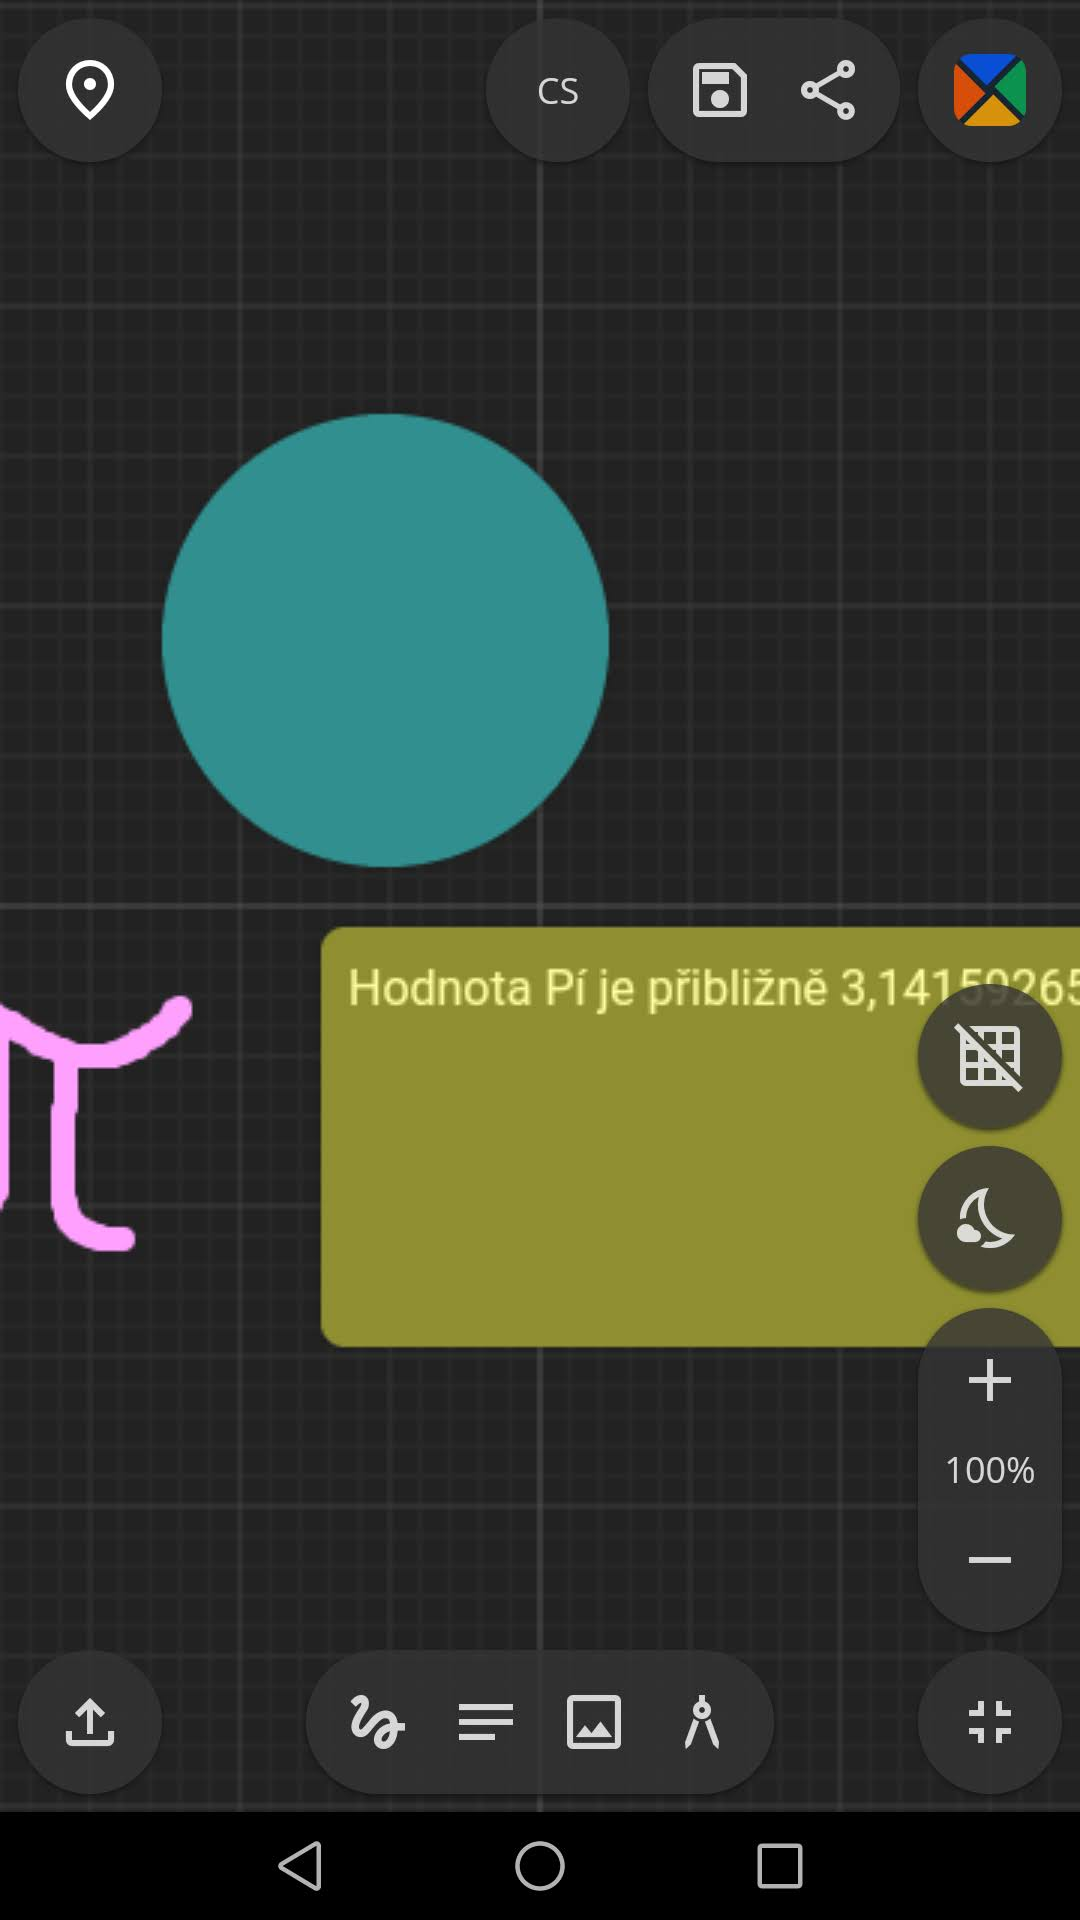
\includegraphics[height=0.5\textwidth, angle=80]{Figures/PhoneVersion.jpg}
        \caption{Obrázek otočený o 80\%}
        \label{fig:graphicx}
    \end{center}
\end{figure}



% Doplnění - sazba not
\section{Sazba not}
\begin{music}
    %\smallmusicsize
    \instrumentnumber{1}
    \setstaffs1{1}
    \generalmeter{\meterC}
    \nobarnumbers
    \startextract
    % bar 1
    \Notes \qu c \en                            % C
    \notes \ibu1d2\qb1d\tbu1\qb1e \en           % beamed DE
    \notes \ibu1g2\qb1f\qb1g%
        \qb1{'a}\tbu1\qb1b \en                  % beamed FGAB
    \bar % bar 2
    \Notes \ql{'c} \en                          % c
    \notes \ibu1{'b}{-3}%
        \qb1b\tbu1\qb1a \en                     % beamed BA
    \notes \ibu1{g}{-3}%
        \qb1g\qb1f\qb1e\tbu1\qb1d \en           % beamed GFED
    \bar % bar 3
    \notes \ibu1f0\qb1c\qb1g\qb1e\tbu1\qb1g%    % beamed CGEG
        \ibu1f0\qb1c\qb1g\qb1e\tbu1\qb1g \en    % beamed CGEG
    \bar % bar 4
    \Notes \qu c\qu e\qu c\qp \en               % CEC
    \endextract
\end{music}



% Doplnění - sazba exotických druhů písma
\section{Sazba exotických druhů písma}
\begin{itemize}
    %\item {\fontfamily{accanthis}\selectfont Písmo Accanthis}
    \item {\fontfamily{calligra}\selectfont Písmo Calligra}
    \item {\punkfamily\selectfont Písmo Punk}
    \item {\foekfamily\selectfont PISMO FOEKFONT}
\end{itemize}
\endinput